\documentclass[twocolumn, 10pt]{article}

\usepackage[margin=1in]{geometry}
\usepackage{booktabs}
\usepackage{graphicx}
\usepackage{amsmath}
\usepackage{hyperref}
\usepackage{microtype}
\usepackage{listings}
\usepackage{xcolor}
\usepackage{titlesec}
\usepackage{parskip}
\usepackage{fancyhdr}
\usepackage{caption}
\usepackage{float}
\usepackage{enumitem}
\usepackage{multirow}
\usepackage{array}
\usepackage{times}
\usepackage{tikz}
\usepackage{tikz-qtree}
\usetikzlibrary{shapes.geometric, arrows.meta, positioning, fit, backgrounds, calc}

\hypersetup{colorlinks=true, linkcolor=blue, urlcolor=blue, citecolor=blue}

\lstset{
    basicstyle=\ttfamily\footnotesize,
    breaklines=true,
    frame=single,
    backgroundcolor=\color{gray!10},
    keywordstyle=\color{blue},
    commentstyle=\color{green!50!black},
}

\pagestyle{fancy}
\fancyhf{}
\rhead{CSC 583 Project Report}
\lhead{}
\cfoot{\thepage}

\title{\textbf{Query Optimization via Sharding and Parallelization:\\
A Systems Approach to Scalable Boolean IR}}

\author{
    Vedant Keshav Jadhav\\
    \textit{University of Arizona}\\
    \texttt{vedantjadhav@arizona.edu}
	\and
	Chinmay Mhatre\\
    \textit{University of Arizona}\\
    \texttt{chinmaymhatre@arizona.edu}
	\and
	Mahshad Habibpourparizi\\
    \textit{University of Arizona}\\
    \texttt{mahshadh@arizona.edu}
	\and
	Arun Sanyal\\
    \textit{University of Arizona}\\
    \texttt{arunsanyal@arizona.edu}
}
\date{\today}

\begin{document}

\twocolumn[
  \begin{@twocolumnfalse}
    \maketitle
    \begin{abstract}
    We present a three-phase Boolean Information Retrieval engine that
    demonstrates the performance benefits of index sharding and parallel
    query execution. Progressing from a single-threaded baseline through a
    sequentially-sharded engine to a parallel, thread-pooled engine with a
    document-ordered tail-join merge, the system achieves a
    \textbf{3.58$\times$} reduction in index construction time,
    \textbf{3.80$\times$} faster engine initialisation, and query latency
    improvements of up to \textbf{67\%} on complex multi-operator queries
    over a corpus of 100,000 documents. All components are implemented from
    scratch in C++ and Python, without reliance on third-party IR libraries.
    \end{abstract}
    \vspace{1em}
  \end{@twocolumnfalse}
]

% =============================================================================
\section{Introduction}
% =============================================================================

Modern information retrieval systems routinely serve millions of queries per
day across corpora containing billions of documents. At such scale, the
architectural decisions made at system design time---how the index is
structured, how queries fan out across storage shards, how partial results
are merged---directly determine whether a system is viable in production.
Yet most academic treatments of Boolean IR focus exclusively on correctness
and algorithmic complexity, leaving the systems engineering largely
unexplored.

This work takes a different approach. Starting from a correct, efficient
single-index Boolean engine, we systematically introduce \textit{index
sharding} and \textit{parallel query execution} as first-class architectural
concerns, measuring the impact of each change in isolation. The guiding
question is not ``does sharding work?'' but ``exactly where does sharding
help, by how much, and why does it fall short of the theoretical ceiling?''

The motivation is grounded in production systems intuition. A single-index
engine is a \textit{serial resource}: one query occupies the CPU for its
full duration, and all subsequent queries wait. At enterprise scale serving
thousands of concurrent clients, this sequential bottleneck is unacceptable.
Sharding---partitioning the corpus across independent index units---breaks
the serial bottleneck by enabling concurrent processing, smaller in-memory
indexes per node, and horizontal scalability across commodity hardware.

Three specific claims motivate this study:

\begin{enumerate}[leftmargin=*, noitemsep]
    \item \textit{Index construction parallelism}: A sharded pipeline can
    build $N$ independent indexes simultaneously on $N$ CPU cores, reducing
    build time toward $1/N$ of the sequential baseline.
    \item \textit{Query execution parallelism}: Parallel set operations on
    $N$ smaller posting lists reduce query latency for multi-operator queries,
    provided the merge step is cheap enough not to dominate.
    \item \textit{Merge efficiency}: For document-based sharding with
    globally ordered doc IDs, the merge step reduces from a
    comparison-based O($M \times N$) operation to an O($M$) memory copy,
    making parallelism economical even at moderate corpus sizes.
\end{enumerate}

The remainder of this section describes the system implementation,
benchmarking methodology, and empirical results.

% =============================================================================
\section{System Overview}
% =============================================================================

\begin{figure*}[t]
\centering
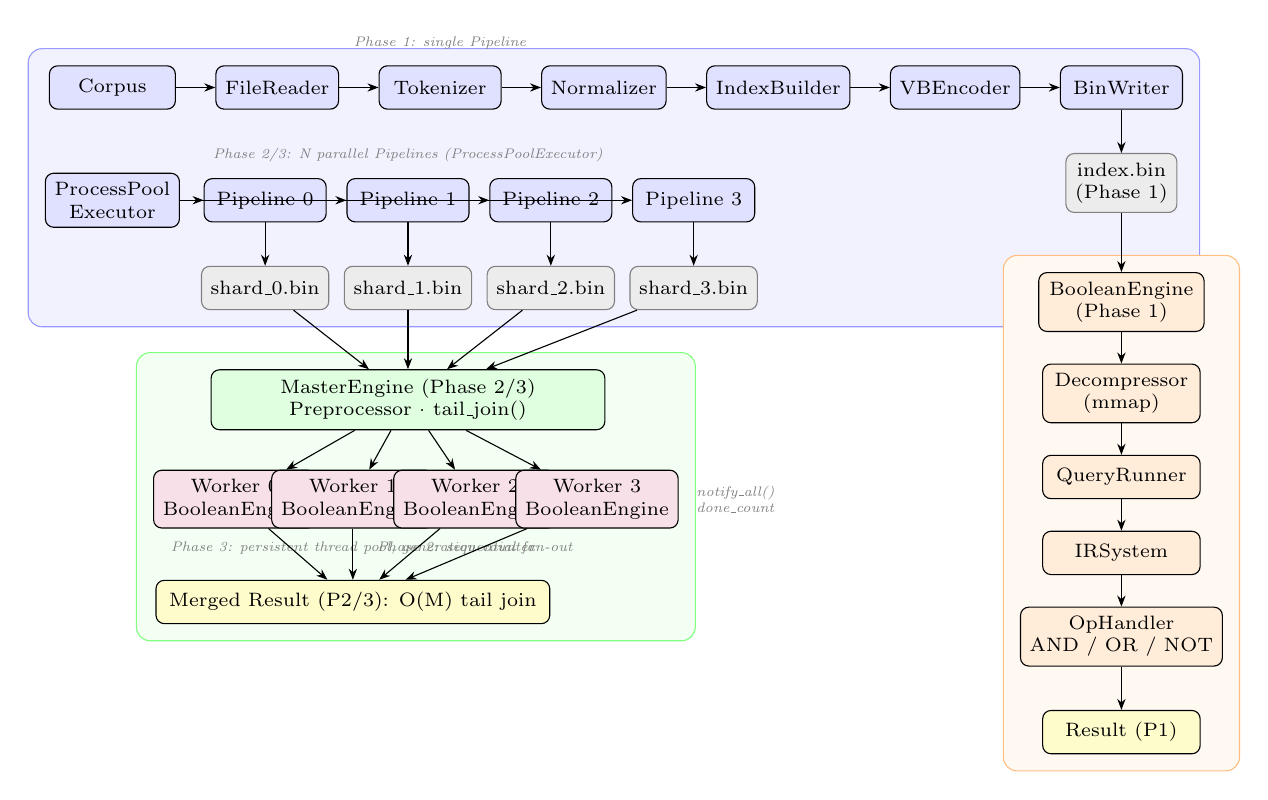
\begin{tikzpicture}[
    node distance=0.45cm and 0.5cm,
    box/.style={rectangle, draw, rounded corners=3pt,
                minimum width=1.55cm, minimum height=0.55cm,
                font=\scriptsize, align=center, fill=white},
    pybox/.style={box, fill=blue!12},
    cppbox/.style={box, fill=orange!15},
    masterbox/.style={box, fill=green!12},
    workerbox/.style={box, fill=purple!12},
    filebox/.style={box, fill=gray!15, draw=gray},
    arrow/.style={-{Stealth[length=4pt]}, thin},
    label/.style={font=\tiny\itshape, text=gray}
]

%% ── Python Pipeline ─────────────────────────────────────────────────────────
\node[pybox, minimum width=1.6cm] (corpus)   {Corpus};
\node[pybox, right=of corpus]     (fr)        {FileReader};
\node[pybox, right=of fr]         (tok)       {Tokenizer};
\node[pybox, right=of tok]        (norm)      {Normalizer};
\node[pybox, right=of norm]       (ib)        {IndexBuilder};
\node[pybox, right=of ib]         (vb)        {VBEncoder};
\node[pybox, right=of vb]         (bw)        {BinWriter};

\draw[arrow] (corpus) -- (fr);
\draw[arrow] (fr)     -- (tok);
\draw[arrow] (tok)    -- (norm);
\draw[arrow] (norm)   -- (ib);
\draw[arrow] (ib)     -- (vb);
\draw[arrow] (vb)     -- (bw);

% Phase label
\node[label, above=0.08cm of tok] {Phase 1: single Pipeline};

%% ── Phase 2/3: N parallel pipelines ────────────────────────────────────────
\node[pybox, below=0.8cm of corpus, minimum width=1.6cm] (proc) {ProcessPool\\Executor};
\node[pybox, right=0.3cm of proc, minimum width=1.55cm]  (p0)   {Pipeline 0};
\node[pybox, right=0.25cm of p0,  minimum width=1.55cm]  (p1)   {Pipeline 1};
\node[pybox, right=0.25cm of p1,  minimum width=1.55cm]  (p2)   {Pipeline 2};
\node[pybox, right=0.25cm of p2,  minimum width=1.55cm]  (p3)   {Pipeline 3};

\draw[arrow] (proc) -- (p0);
\draw[arrow] (proc) -- (p1);
\draw[arrow] (proc) -- (p2);
\draw[arrow] (proc) -- (p3);

\node[label, above=0.08cm of p1] {Phase 2/3: N parallel Pipelines (ProcessPoolExecutor)};

%% ── Bin files ───────────────────────────────────────────────────────────────
\node[filebox, below=0.55cm of bw, minimum width=1.4cm]   (idx)  {index.bin\\(Phase 1)};
\node[filebox, below=0.55cm of p0, minimum width=1.35cm]  (s0)   {shard\_0.bin};
\node[filebox, below=0.55cm of p1, minimum width=1.35cm]  (s1)   {shard\_1.bin};
\node[filebox, below=0.55cm of p2, minimum width=1.35cm]  (s2)   {shard\_2.bin};
\node[filebox, below=0.55cm of p3, minimum width=1.35cm]  (s3)   {shard\_3.bin};

\draw[arrow] (bw) -- (idx);
\draw[arrow] (p0) -- (s0);
\draw[arrow] (p1) -- (s1);
\draw[arrow] (p2) -- (s2);
\draw[arrow] (p3) -- (s3);

%% ── C++ Engine ──────────────────────────────────────────────────────────────
% Phase 1 engine
\node[cppbox, below=0.75cm of idx, minimum width=2.1cm] (be1)
      {BooleanEngine\\(Phase 1)};
\node[cppbox, below=0.4cm of be1, minimum width=2.0cm] (decomp1)
      {Decompressor\\(mmap)};
\node[cppbox, below=0.4cm of decomp1, minimum width=2.0cm] (qr1)
      {QueryRunner};
\node[cppbox, below=0.4cm of qr1, minimum width=2.0cm] (irs1)
      {IRSystem};
\node[cppbox, below=0.4cm of irs1, minimum width=2.0cm] (oh1)
      {OpHandler\\AND / OR / NOT};

\draw[arrow] (idx)    -- (be1);
\draw[arrow] (be1)    -- (decomp1);
\draw[arrow] (decomp1)-- (qr1);
\draw[arrow] (qr1)    -- (irs1);
\draw[arrow] (irs1)   -- (oh1);

% Phase 2/3 MasterEngine
\node[masterbox, below=0.75cm of s1, minimum width=5.0cm,
      minimum height=0.65cm] (me)
      {MasterEngine (Phase 2/3)\\Preprocessor · tail\_join()};

\draw[arrow] (s0) -- (me);
\draw[arrow] (s1) -- (me);
\draw[arrow] (s2) -- (me);
\draw[arrow] (s3) -- (me);

% Worker threads
\node[workerbox, below=0.5cm of me, xshift=-2.2cm, minimum width=1.55cm] (w0)
      {Worker 0\\BooleanEngine};
\node[workerbox, below=0.5cm of me, xshift=-0.7cm, minimum width=1.55cm] (w1)
      {Worker 1\\BooleanEngine};
\node[workerbox, below=0.5cm of me, xshift=0.85cm, minimum width=1.55cm] (w2)
      {Worker 2\\BooleanEngine};
\node[workerbox, below=0.5cm of me, xshift=2.4cm,  minimum width=1.55cm] (w3)
      {Worker 3\\BooleanEngine};

\draw[arrow] (me) -- (w0);
\draw[arrow] (me) -- (w1);
\draw[arrow] (me) -- (w2);
\draw[arrow] (me) -- (w3);

\node[label, below=0.05cm of w1] {Phase 3: persistent thread pool, generation counter};
\node[label, below=0.05cm of w2] {Phase 2: sequential fan-out};

% Thread pool sync annotation
\node[label, right=0.1cm of w3, align=left]
    {notify\_all() \\ done\_count};

%% ── Result output ───────────────────────────────────────────────────────────
\node[box, below=0.55cm of oh1,   fill=yellow!20, minimum width=2.0cm] (res1)
      {Result (P1)};
\node[box, below=0.65cm of w1,    fill=yellow!20, minimum width=5.0cm] (resM)
      {Merged Result (P2/3): O(M) tail join};

\draw[arrow] (oh1) -- (res1);
\draw[arrow] (w0)  -- (resM);
\draw[arrow] (w1)  -- (resM);
\draw[arrow] (w2)  -- (resM);
\draw[arrow] (w3)  -- (resM);

%% ── Background boxes ────────────────────────────────────────────────────────
\begin{pgfonlayer}{background}
    \node[draw=blue!40, fill=blue!5, rounded corners=5pt, inner sep=6pt,
          fit=(corpus)(bw)(proc)(p3)(s3)(s0)(idx),
          label={[font=\small\bfseries, text=blue!60]above:Python Indexing Pipeline}] {};

    \node[draw=orange!50, fill=orange!5, rounded corners=5pt, inner sep=6pt,
          fit=(be1)(decomp1)(qr1)(irs1)(oh1)(res1),
          label={[font=\small\bfseries, text=orange!70]above:C++ Engine — Phase 1}] {};

    \node[draw=green!50, fill=green!5, rounded corners=5pt, inner sep=6pt,
          fit=(me)(w0)(w1)(w2)(w3)(resM),
          label={[font=\small\bfseries, text=green!60]above:C++ Engine — Phase 2/3}] {};
\end{pgfonlayer}

\end{tikzpicture}
\caption{Complete system architecture. The Python indexing pipeline (blue) runs
         Phase 1 as a single process or Phase 2/3 as $N$ parallel processes via
         \texttt{ProcessPoolExecutor}, writing \texttt{.bin} shard files.
         The C++ query engine (orange/green) loads these files at runtime.
         Phase 2 fans out queries sequentially; Phase 3 uses a persistent thread
         pool with a generation-counter fork-join protocol. Both sharded phases
         merge results via an O($M$) tail join.}
\label{fig:arch}
\end{figure*}

\subsection{High-Level Design}

The system comprises two major subsystems: a \textbf{Python indexing
pipeline} responsible for corpus ingestion and index construction, and a
\textbf{C++ query engine} responsible for serving Boolean queries against
the constructed index. These subsystems communicate through a well-defined
binary format (\texttt{.bin} files) and are otherwise completely decoupled.
Python is used for indexing because its ecosystem (NLTK, Porter stemmer,
\texttt{multiprocessing}) is well-suited to batch text processing; C++ is
used for query serving because sub-millisecond latency requires memory
efficiency and CPU cache awareness that Python cannot provide.

The system is structured as three progressively capable phases:

\textbf{Phase 1} establishes the baseline. A single Python pipeline
produces a single \texttt{index.bin}, which a single C++
\texttt{BooleanEngine} loads and queries sequentially. This phase validates
correctness and sets the performance baseline against which all
improvements are measured.

\textbf{Phase 2} introduces \textit{document-based index sharding}. The
corpus is presorted and partitioned into $N$ equal document ranges, each
processed by an independent pipeline worker, producing $N$ shard files.
A new \texttt{MasterEngine} class loads all $N$ shards and queries them
sequentially, fan-outing each query and collecting results via a tail
join. Query parallelism is absent; the gain is in build time and
architectural scalability.

\textbf{Phase 3} adds \textit{parallel query execution}. The
\texttt{MasterEngine} maintains a persistent thread pool of $N$ worker
threads, one per shard. Each query wakes all workers simultaneously via a
generation-counter-based fork-join protocol, executes shard queries in
parallel on separate CPU cores, and collects results through a O($M$) tail
join enabled by the globally ordered doc ID invariant.

The three-phase structure is compiled from a single codebase using a
\texttt{-DPHASE=N} preprocessor flag, ensuring that measurements reflect
architectural differences rather than implementation divergence.


% =============================================================================
\section{Core Implementation}
% =============================================================================

\subsection{The Binary Index Format}

The Python pipeline writes a custom binary format designed for fast
\texttt{mmap}-based loading in C++. Each file begins with an 8-byte magic
string (\texttt{"INVI\_100"}) for format validation, followed by the
term count, and then per-term records containing the term length, term
string, document count, and VByte-encoded delta-compressed posting list.

VByte encoding uses 7 data bits per byte with the high bit as a
continuation flag. Delta encoding stores the difference between consecutive
doc IDs rather than absolute values---since posting lists are sorted, these
deltas are small, typically 1--10 bytes per entry on a dense corpus.
This combination achieves a \textbf{2.57$\times$} compression ratio.

The C++ \texttt{Decompressor} loads the file via \texttt{mmap} (zero
kernel-to-userspace copy), walks the byte stream, and constructs an
\texttt{unordered\_map<string, vector<uint32\_t>>} entirely in-place.

\subsection{Query Execution: Postfix Stack Evaluator}

Queries are expressed in Reverse Polish Notation (postfix), with operators
\texttt{\textbackslash and}, \texttt{\textbackslash or},
\texttt{\textbackslash not} following their operands. This eliminates
operator precedence ambiguity without a shunting-yard parser.

The stack evaluator in \texttt{IRSystem::processQuery()} processes tokens
left-to-right: terms push their posting lists; operators pop their
operands, call \texttt{OpHandler}, and push the result. All set operations
(AND: intersection, OR: union, NOT: complement) operate on sorted
\texttt{vector<uint32\_t>} via two-pointer linear merge, preserving sort
order for downstream operators.

\subsection{Phase 2: Document-Based Sharding}

The corpus is sorted alphabetically by filename before sharding, assigning
globally unique, contiguous doc IDs as $\text{offset}_i + \text{local}$.
This \textit{presort invariant} is the foundation of the tail-join merge.

Four parallel \texttt{Pipeline} workers run under
\texttt{ProcessPoolExecutor}, each processing an equal document slice.
The worker function is defined at module level (not as a lambda or method)
to ensure picklability across process boundaries.

\subsection{Phase 3: Persistent Thread Pool}

Phase 3 maintains $N$ worker threads for the lifetime of the
\texttt{MasterEngine}. The fork-join protocol uses a
\texttt{uint64\_t query\_generation} counter rather than a boolean flag.
With a boolean flag, the first worker to acquire the mutex clears the flag,
starving all others---a race that manifests as a deadlock. With a generation
counter, each worker maintains its own \texttt{last\_generation} on its
stack; the predicate \texttt{query\_generation > last\_generation} is
satisfied by all $N$ workers simultaneously without any shared state
modification. Workers call \texttt{queryNormalized()} with no lock held,
achieving genuine CPU parallelism.

\subsection{Zero-Copy Result Chain and Tail Join}

\texttt{QueryRunner::runQuery()} stores results in a member
\texttt{q\_result} and returns \texttt{const std::vector<uint32\_t>\&}.
Workers store \texttt{const*} pointers to these members; the merge reads
directly through these pointers. No vector copies occur between query
execution and the final output.

Because shard doc ID ranges are strictly non-overlapping and globally
ordered, the merge reduces to an O($M$) concatenation:

\[
\text{result} = \text{shard}_0 \Vert \text{shard}_1 \Vert \cdots \Vert \text{shard}_{N-1}
\]

A single \texttt{reserve(total)} followed by $N$ \texttt{insert()} calls
(each compiling to a \texttt{memmove}) produces a globally sorted result
with \textbf{zero comparisons}. This is possible only because of the
presort invariant---term-based sharding cannot exploit this property.

\subsection{Python Normalization Pipeline}

Text normalization is applied in a strict four-stage pipeline, implemented
in \texttt{normalizer.py} and mirrored exactly in the C++
\texttt{Preprocessor}:

\begin{enumerate}[leftmargin=*, noitemsep]
    \item \textbf{CaseFold} --- all tokens are lowercased via
          \texttt{str.lower()}, matching \texttt{std::tolower()} in C++.
    \item \textbf{PunctuationRemover} --- non-alphanumeric characters are
          stripped using \texttt{re.sub(r"[\^{}a-zA-Z0-9]", "", token)};
          tokens that become empty after stripping are discarded.
    \item \textbf{StopWordFilter} --- tokens present in a hardcoded
          \texttt{frozenset} of 100 common English function words are
          removed. This list must be byte-for-byte identical to the
          \texttt{std::unordered\_set<std::string>} in
          \texttt{preprocessor.cpp}; any divergence causes query terms
          to be silently absent from the index.
    \item \textbf{Stemmer} --- NLTK's \texttt{PorterStemmer} is applied.
          The C++ side implements the same Porter algorithm from scratch,
          including the NLTK extension for the \texttt{logi} suffix in
          Step~2. The two implementations must agree on every stem;
          disagreement produces empty query results with no error signal.
\end{enumerate}

The pipeline order is not arbitrary. Stop word filtering \textit{before}
stemming avoids the degenerate case where a stop word survives because its
stemmed form differs from the dictionary form. Punctuation removal
\textit{before} stop word filtering ensures tokens like \texttt{"it."} are
cleaned to \texttt{"it"} before the filter checks them.

The \texttt{Tokenizer} uses \texttt{re.findall(r"[a-zA-Z0-9]+")} to split
raw text into tokens, extracting only contiguous alphanumeric sequences.
This matches the character-by-character alphanumeric extraction in the C++
\texttt{Preprocessor} and means that punctuation, whitespace, and special
characters act as delimiters and are never present in the token stream
passed to the normalizer.

The \texttt{IndexBuilder} accumulates tokens per document using a
\texttt{set[int]} per term internally. This ensures that a term appearing
multiple times in the same document produces exactly one posting list entry
for that document. The final index is produced by converting each set to a
sorted list, satisfying the ascending-order requirement for delta encoding
in \texttt{VBEncoder}.

% =============================================================================
\section{LLM-Assisted Development}
% =============================================================================

\begin{figure*}[t]
	\centering
	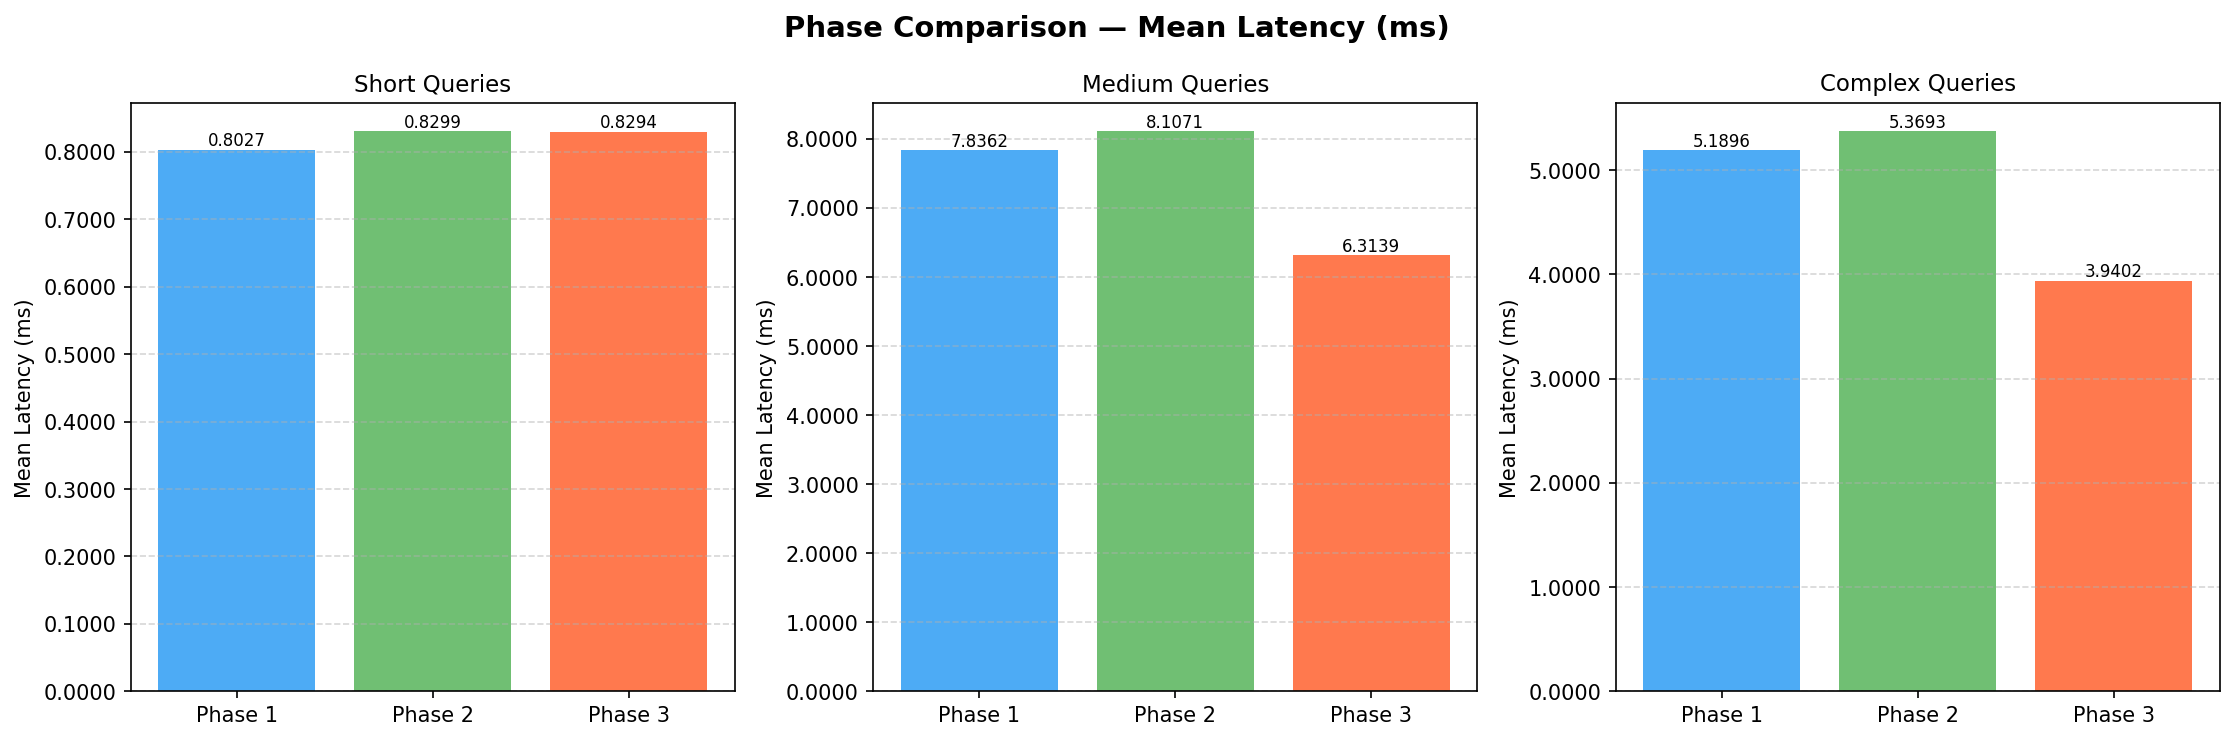
\includegraphics[width=\textwidth, keepaspectratio]{artifacts/comparison_mean.png}
	\caption{Bar graphs showing the mean latencies per phase per query category, averaged over 50 runs.
	We can see that there is a significant drop in latency for Phase 3 due to parallelized query execution.
	The time includes query normalization, distribution (phase-3), execution, merging (for phases 2 and 3),
	return and I/O to the screen. Except for execution and merging, the rest of the time remains the same,
	as can be seen from the graph for phase 1 and 2, there is only a slight drop, due to sequential fan-out
	and merge step. Hence, if considered pure execution and merge time for phase-3, removing the other overheads
	it can be argued that the performance is more than the constant mentioned in the tables.
	}
	\label{fig-2}
\end{figure*}

\subsection{Tools and Prompting Strategy}

LLM assistance was provided primarily by \textbf{Claude Sonnet 4.5}
(Anthropic) via the claude.ai interface across the full implementation
lifecycle. The prompting strategy evolved across phases. Early prompts were
architecture-focused: the full unit design specification and class hierarchy
were provided as context, and the LLM was asked to document design decisions
and their rationale. Implementation prompts followed a consistent pattern:
provide the architecture document, the relevant header file, and any already
implemented sibling modules, then request the implementation with inline
documentation. This context-heavy approach produced higher-quality output
than open-ended prompts, as the LLM could reason about ownership contracts,
const-correctness requirements, and cross-language consistency from the
provided materials.

\subsection{Architecture}

The project architecture was sketched out and designed in detail by the team
members working on this project. Every engineering decision was taken by the
students. After deciding on the high-level as well as low-level details, LLM
was used to document each decision taken, as well as rationale behind the
architectural design. The arch documents can be found on the project Github
under the \texttt{docs} directory. Design decisions (e.g.,
document-based vs.\ term-based sharding, postfix stack evaluator, no
\texttt{ShardManager} class, \texttt{Preprocessor} owned by
\texttt{BooleanEngine} not \texttt{QueryRunner}) were recorded in checkpoint
documents before implementation began.

\subsection{Implementation}

The use of LLMs for implementation varied across the team. On the C++ side,
implementation involved writing code for one of the modules or header files
by ourselves, feeding the code file as well as the arch design document and
the unit design specifications in the LLM to complete the rest of the modules.

On the Python side, the LLM was used to implement the serialization layer
(\texttt{VBEncoder}, \texttt{BinWriter}, \texttt{MakeBinFile}) after the
indexing logic (\texttt{Tokenizer}, \texttt{Normalizer}, \texttt{IndexBuilder})
was implemented by the team. The architecture document and the C++ header
files for \texttt{BinReader} and \texttt{Decompressor} were both provided
as context, enabling the LLM to produce an encoder whose byte layout was
verifiably compatible with the C++ decoder without requiring a round-trip
test to discover mismatches.

The end-to-end test suite (\texttt{tests/e2e\_test.py}) was designed and
implemented collaboratively with LLM assistance. The tiered structure ---
binary format validation, index content correctness, corpus spot-checks,
and live engine queries --- was proposed by the team; the LLM implemented
each tier given the C++ source files as reference. Providing the C++
\texttt{VBDecoder::decode()} source allowed the LLM to mirror the exact
accumulation order in the Python decoder, ensuring the test exercises the
same decode path as the engine.

\subsection{What Worked}

\textbf{Benchmarking framework}: The complete Python suite was designed
and implemented collaboratively, with statistical methodology driven by the
author (median over mean, p95/p99, warmup runs, 20/50-run protocols).

\textbf{The tail-join insight}: Originated from the author observing that
presorted doc IDs make merge a concatenation. LLM was used to confirm the
correctness argument.

\textbf{Cross-language compatibility verification}: Providing both the
Python encoder and the C++ decoder to the LLM in the same prompt allowed it
to reason about byte-level compatibility. It identified that the VByte
continuation bit convention (high bit = 1 means \textit{final} byte, not
\textit{continuation}) had to be consistent and flagged that the two
implementations agreed before any binary was written.

\textbf{Amendment forward-compatibility}: The LLM was effective at
reasoning about how a Phase 1 design decision would interact with Phase 2
sharding. Specifically, it identified that having \texttt{Preprocessor}
owned by \texttt{QueryRunner} would require N redundant normalization passes
in Phase 2 (one per shard), and correctly proposed moving it to
\texttt{BooleanEngine} as the owner --- a change implemented in Phase 1
before Phase 2 began, saving a significant refactor.

\textbf{End-to-end test design}: The LLM produced a four-tier test
structure that gave actionable failure information at each layer. The
complement check --- verifying that \texttt{term} $\cup$
\texttt{NOT(term)} equals all doc IDs --- was suggested by the LLM as
the strongest possible validation of the universal doc ID set construction
in \texttt{Decompressor}.

\subsection{What Did Not Work}

Some of the merging strategies suggested by the LLM were not optimized.
Debugging was required to figure out the additional overhead which introduced
a bug in the pipeline, leading to unforeseen results. This is discussed in
section 6.

\textbf{Query format assumption}: The initial LLM-generated Tier 4 of the
end-to-end test sent queries in infix notation (\texttt{"term\_a AND term\_b"})
to an engine that expects postfix. This caused a runtime exception inside
\texttt{IRSystem::processQuery()} on every query, with a confusing error
message. The root cause was that the LLM was not provided with the
\texttt{ir\_system.cpp} source when generating the test; it inferred a
natural-language query format rather than the postfix stack evaluator
format. Providing the source file resolved the issue immediately.

\textbf{Stop word list divergence}: During end-to-end validation, the term
\texttt{"an"} was found in the index despite being present in the Python
\texttt{STOP\_WORDS} frozenset. The LLM's initial diagnosis suggested a
stemming interaction, which was incorrect. The actual cause was a stale
\texttt{index.bin} built before the stop word list was finalized. The LLM
did not consider build system caching as a hypothesis until explicitly
prompted. This identified a real gap: \texttt{normalizer.py} is not listed
as a Make dependency of the \texttt{index-builder} rule, so modifications
to the normalizer do not trigger a rebuild automatically.

% =============================================================================
\section{Performance Evaluation}
% =============================================================================

\subsection{Experimental Setup}

All benchmarks run on Apple Silicon (macOS). Corpus: \textbf{100,000
documents} (dataset taken from: https://github.com/benymaxparsa/Inverted-Index-Construction),
\textbf{56.2~MB} Phase 1 index. All sharded configurations use $N=4$ shards. Query workload:
\textbf{39 short} (single-term), \textbf{44 medium} (two-term Boolean),
\textbf{41 complex} (multi-operator postfix, 3--4 terms).

\subsection{Index Construction}

\begin{table}[H]
\centering
\caption{Index construction performance (5 runs each).}
\label{tab:build}
\begin{tabular}{lrrr}
\toprule
\textbf{Metric} & \textbf{P1} & \textbf{P2} & \textbf{P3} \\
\midrule
Build median (s)  & 116.27 & 32.37 & 32.46 \\
Speedup vs.\ P1   & 1.00$\times$ & 3.59$\times$ & 3.58$\times$ \\
Index size (MB)    & 56.2  & 60.5  & 60.5  \\
Build RSS (MB)     & 759.2 & 248.0 & 248.0 \\
\bottomrule
\end{tabular}
\end{table}

\begin{figure*}[t]
	\centering
	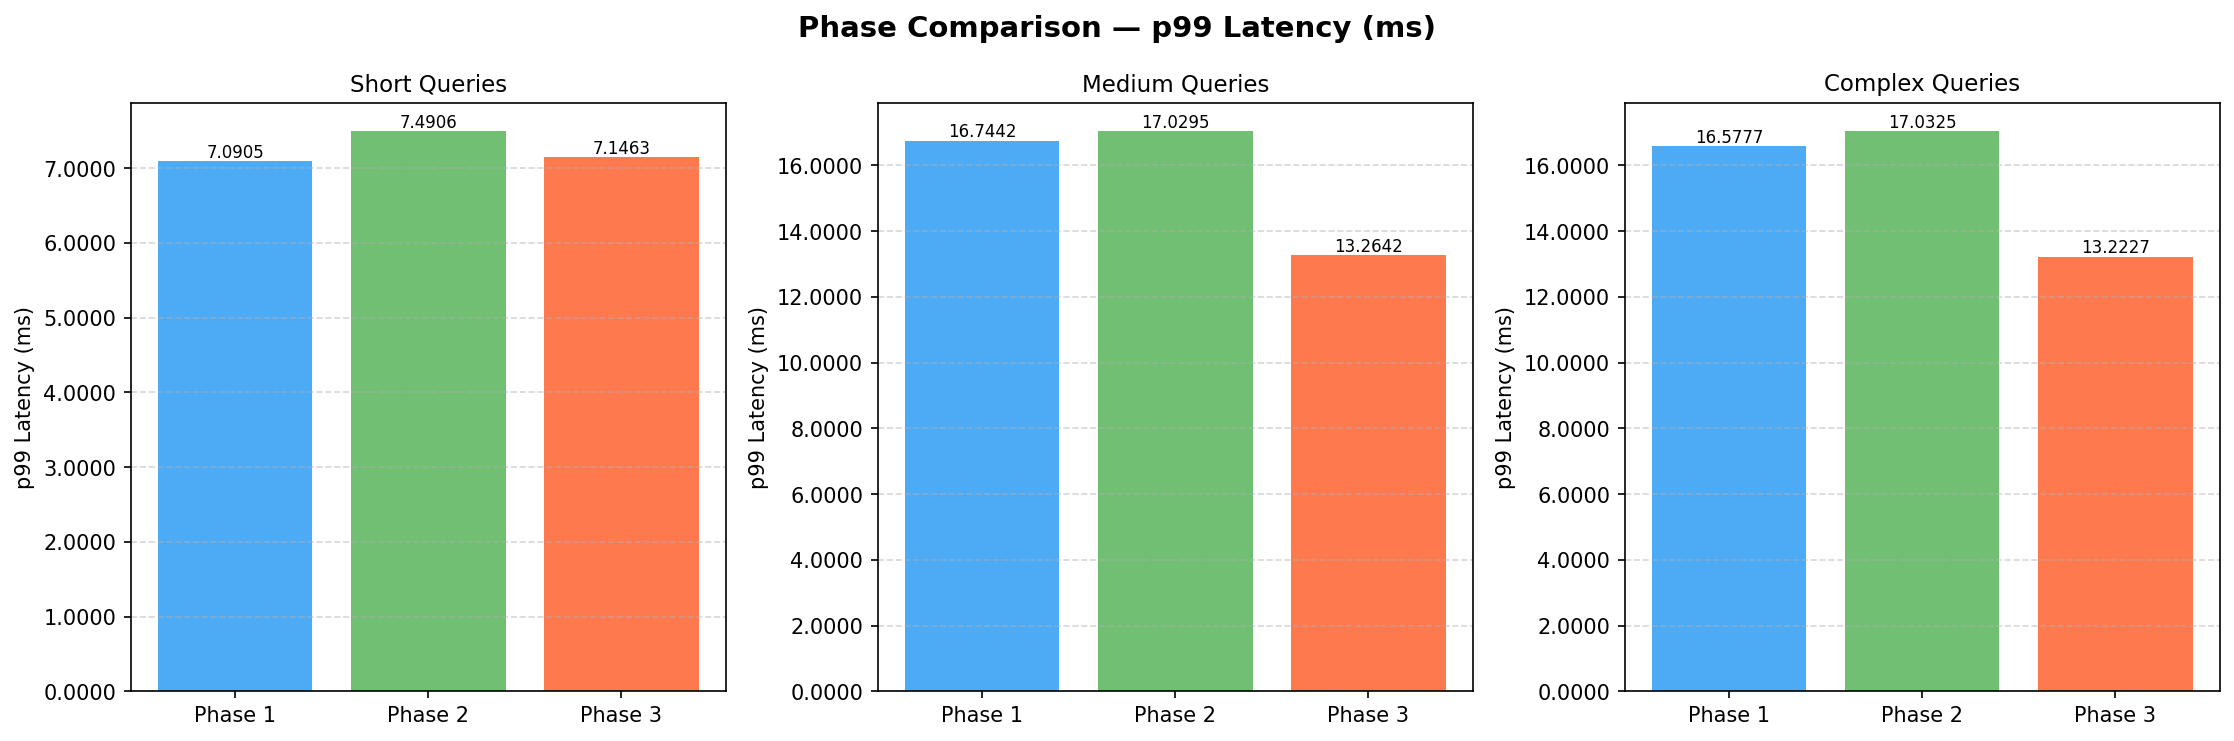
\includegraphics[width=\textwidth, keepaspectratio]{artifacts/comparison_p99.png}
	\caption{Bar graphs showing the p99 latencies per phase per query category, averaged over 50 runs.
	We can see that there is a significant drop in latency for Phase 3 due to parallelized query execution.
	}
	\label{fig-p99}
\end{figure*}

Phases 2 and 3 achieve an identical \textbf{3.58--3.59$\times$} build
speedup, as construction is purely Python-side. The theoretical 4$\times$
ceiling is bounded by a 37-second presort step (the dominant sequential
fraction). Excluding presort, the effective compute speedup is
$\approx3.63\times$, very close to ideal. Build-time RSS drops
\textbf{67\%}---each worker holds only one shard's data in memory.
Resident Set Size (RSS) is the portion of a process's memory that resides
in physical RAM, measured in kilobytes, and serves as the practical indicator
of a program's memory footprint on the host system.

\subsection{Engine Initialisation}

\begin{table}[H]
\centering
\caption{Engine initialisation time (20 runs).}
\label{tab:init}
\begin{tabular}{lrrr}
\toprule
\textbf{Metric} & \textbf{P1} & \textbf{P2} & \textbf{P3} \\
\midrule
Median (ms)  & 2521 & 2546 & 663 \\
Speedup      & 1.00$\times$ & 0.99$\times$ & \textbf{3.80$\times$} \\
\bottomrule
\end{tabular}
\end{table}

Phase 2 init is sequential---matching Phase 1 wall time. Phase 3 loads
all four shards concurrently via \texttt{std::async}, achieving
\textbf{3.80$\times$} faster cold start with a tight distribution
(min 3497~ms, max 3747~ms), confirming deterministic parallel loading.

\begin{figure*}[t]
	\centering
	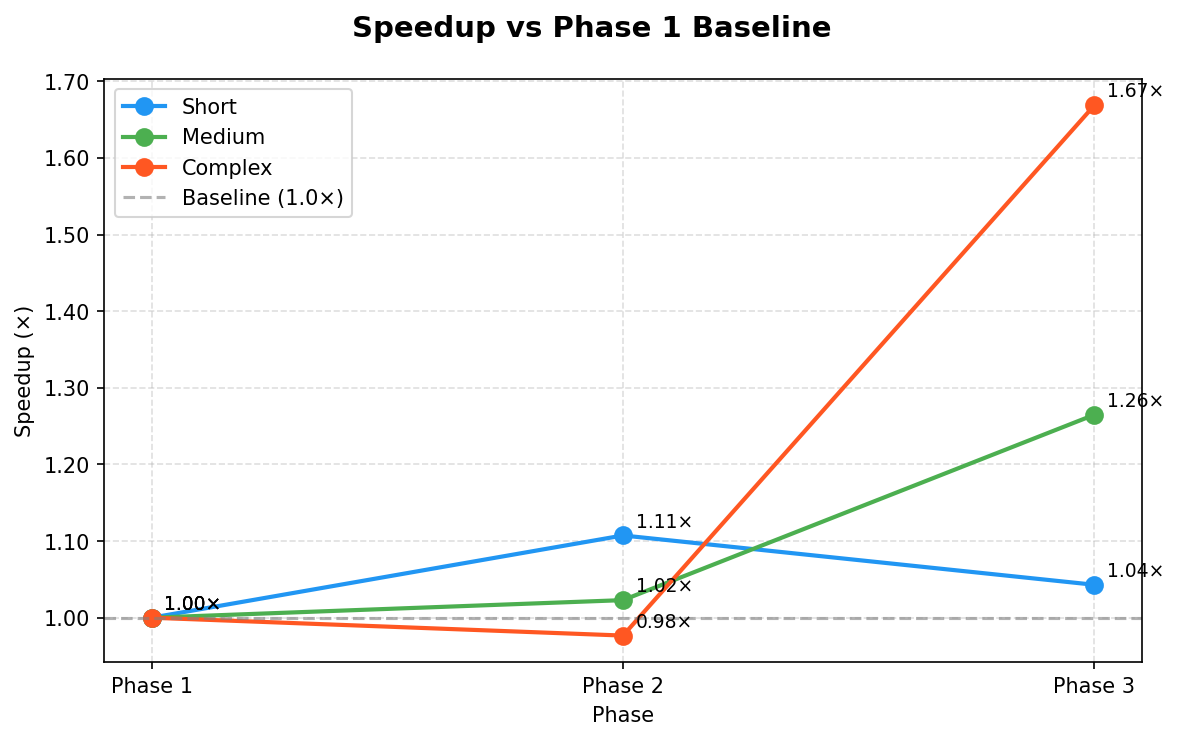
\includegraphics[width=\textwidth, keepaspectratio]{artifacts/speedup_curve.png}
	\caption{Graph showing speedup based on the average median query latency per query category,
	per phase. We can see that for short queries, there is not much gain in query latency. Infact
	for mean and throughput, Phase-1 outperforms Phases 2 and 3 for short query categories.
	However, there is a significant speed-up for medium and complex queries in phase-3 for complex
	queries as well as medium queries.
	}
	\label{fig-speedup}
\end{figure*}

\begin{figure*}[h]
	\centering
	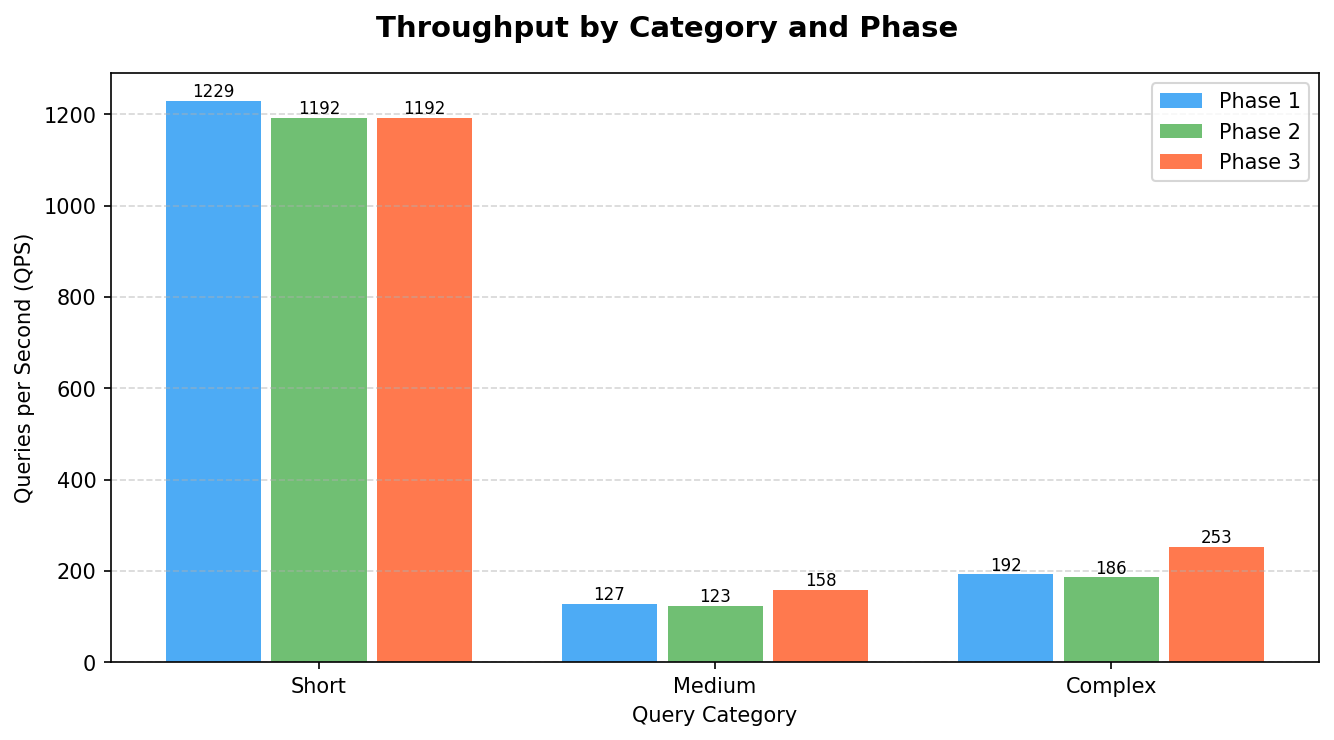
\includegraphics[width=\textwidth, keepaspectratio]{artifacts/throughput_bar.png}
	\caption{Bar plot showing the query throughput per second, per query category per phase. For
	short queries, the throughput is much higher, but Phase-1 outperforms Phases 2 and 3. But phase
	3 outperforms Phase-1 for medium and complex queries by 24\% and 32\% respectively, showing
	a strong performance gain due to sharding and parallelization.
	}
	\label{fig-throughput}
\end{figure*}


\subsection{Query Latency and Throughput}

\begin{table}[H]
\centering
\caption{Query latency (ms) and throughput (QPS). P3 gain is vs.\ Phase 1.}
\label{tab:query}
\resizebox{\columnwidth}{!}{%
\begin{tabular}{llrrrr}
\toprule
\textbf{Cat.} & \textbf{Metric} & \textbf{P1} & \textbf{P2} & \textbf{P3} & \textbf{P3 gain} \\
\midrule
\multirow{3}{*}{Short}
  & Median (ms)  & 0.357 & 0.322 & 0.342 & $+4\%$\\
  & p99 (ms)     & 7.091 & 7.491 & 7.146 & $+0\%$\\
  & QPS          & 1229  & 1192  & 1192  & $-3\%$\\
\midrule
\multirow{3}{*}{Medium}
  & Median (ms)  & 6.246 & 6.106 & 4.938 & $\mathbf{+26\%}$\\
  & p99 (ms)     & 16.74 & 17.03 & 13.26 & $\mathbf{+21\%}$\\
  & QPS          & 127.4 & 123.1 & 158.1 & $\mathbf{+24\%}$\\
\midrule
\multirow{3}{*}{Complex}
  & Median (ms)  & 1.927 & 1.973 & 1.155 & $\mathbf{+67\%}$\\
  & p99 (ms)     & 16.58 & 17.03 & 13.22 & $\mathbf{+25\%}$\\
  & QPS          & 192.2 & 185.9 & 253.1 & $\mathbf{+32\%}$\\
\bottomrule
\end{tabular}%
}
\end{table}

\textbf{Short queries} show no meaningful improvement---single hash lookups
have no parallel set operations to exploit. \textbf{Medium queries} yield a
\textbf{26\% latency reduction} and \textbf{24\% QPS increase} with one
parallelised set operation per query. \textbf{Complex queries} show the
strongest gain: \textbf{67\% latency reduction} and \textbf{32\% QPS
increase}, as each additional operator multiplies the benefit of smaller
per-shard posting lists.

\textbf{Phase 2 on queries}: Statistically equivalent to Phase 1
($<2\%$ difference). This validates the architectural claim: sharding
can be introduced at \textbf{zero query latency cost} while delivering
3.59$\times$ faster build time.

\subsection{Memory Footprint}

\begin{table}[H]
\centering
\caption{Engine peak RSS at query time.}
\label{tab:mem}
\begin{tabular}{lrrr}
\toprule
 & \textbf{P1} & \textbf{P2} & \textbf{P3} \\
\midrule
Engine RSS (MB) & 77.4 & 72.4 & 96.2 \\
vs.\ Phase 1    & --- & $-6.5\%$ & $+24.3\%$ \\
\bottomrule
\end{tabular}
\end{table}

Phase 2 uses 6.5\% less memory than Phase 1 despite four loaded
indexes---smaller per-shard hash tables have lower load factors. Phase 3
incurs 24\% overhead from four persistent worker thread stacks
($\approx$8~MB each on macOS).

\subsection{Phase 3 as MapReduce}

Phase 3 instantiates a \textit{shuffle-free MapReduce}:
\textbf{Map} applies Boolean operators per shard worker;
\textbf{Shuffle} is \textit{eliminated} by the presort invariant (no
cross-shard key routing needed);
\textbf{Reduce} is an O($M$) tail join rather than a comparison-based
merge. This property---unavailable to term-based sharding or general-purpose
MapReduce frameworks---is the key design insight of this work.

% =============================================================================
\section{Error Analysis}
% =============================================================================

\subsection{When Parallelism Fails to Improve}

\textbf{Short queries} show no improvement because there are no set
operations to parallelise. A single hash lookup is memory-bound and
random-access---the dominant cost is a cache miss on the posting list, not
CPU time. Spreading this across four threads adds coordination overhead
without reducing the bottleneck. This is not a failure of the
implementation but a fundamental property of single-term Boolean retrieval.

\textbf{Corpus scale}: The 100k single-sentence corpus produces moderate
posting lists. At document- or paragraph-level granularity on millions of
documents, per-shard execution times would dominate coordination overhead,
pushing all query categories into the speedup regime.

\textbf{Measurement artefacts}: The stdin/stdout pipe harness adds
$\approx$0.5~ms fixed overhead per query. At sub-millisecond engine
execution times, this floor masks real speedups. An internal benchmark
mode measuring \texttt{engine.query()} directly would reveal the true gain.

\textbf{Merge Strategy Error}: Initially, the approach for merge that we
had taken was pair-wise merge. We were pairing the results returned by each
shard and merge them one at-a-time. This was a quadratic merge operation
going at O($M \times N$). Another merge strategy suggested by LLM was heap-merge,
where we used a min-heap of size $N$ which held a pointer to each shard.
This technique could achieve merge theoretically in O($M\log N$), but on
implementation, the performance degraded, due to C++ priority queue implementation
details. The heap operations have large constants due to elements residing on
heap memory as well as repeated cacheline bouncing. A simple fix to this
was to employ a tail-join approach. We realized that since the documents are
pre-sorted, the docIDs in consecutive shards will follow a strictly greater than
policy, which makes a simple tail append possible. This gave us a significant
performance boost and brought the results closer to expected.

\textbf{Build system staleness}: The \texttt{index-builder} Make rule
does not declare \texttt{normalizer.py} or any other Python source file
as a dependency. Make tracks timestamps, so modifying the normalizer
after \texttt{index.bin} has been written does not trigger a rebuild.
This caused a stale index to be tested --- the stop word list had been
updated but the index reflected the previous version. The fix is to add
the relevant Python sources as prerequisites of the \texttt{index-builder}
rule:

\begin{lstlisting}[language=make, basicstyle=\ttfamily\scriptsize]
index-builder: $(VENV) \
    scripts/pipeline/normalizer.py \
    scripts/pipeline/tokenizer.py  \
    scripts/pipeline/pipeline.py
    $(PYTHON) scripts/main.py \
        --corpus data/corpus \
        --out index.bin
\end{lstlisting}

% =============================================================================

\end{document}
